\subsection{溶液饱和温度、溶解度和过饱和度的测定}
溶液到达饱和状态时的温度,即溶质固体和溶液达成平衡的温度称为溶液的饱和温度。准确地测定溶液的饱和温度是搞好下种操作的前提,也是测定溶解度和过饱和度的基础,所以饱和温度的测定是从溶液中培养晶体的一项基本功。常用的测定饱和温度的方法有以下几种:

\paragraph{(1) 平衡法}
在接近饱和的溶液中,放人一些溶质固体,在一定温度下不断搅拌,直到溶液中尚余少量固体不再溶解为止,此时溶液的温度即可看成是溶液的饱和温度。这个方法虽然简便,但要达到真正平衡所需的要达到真正平衡所需的时间较长(约数小时至数天,视溶液的粘度和搅拌强度而定),而且精确度也较低,约0.5—1℃。

\paragraph{(2) 浓度涡流法}
\begin{figure}[thb]
 \centering
 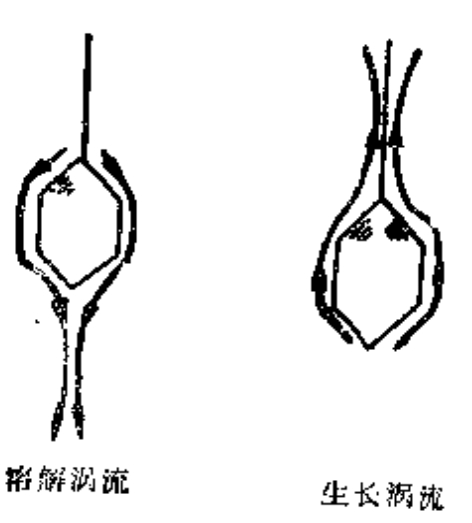
\includegraphics[width=0.4\textwidth]{fig/cp03/img3.8.jpg}
 \caption{浓度涡流。}
\end{figure}
%TODO:Fig.3.8
用尼龙线将一小块晶体悬在其接近饱和温度的溶液中,仔细观察晶体及其附近的液流情况。如果溶液是不饱和的,则晶体稜角变得圆滑。靠近晶体表面的溶液,由于晶体的溶解,其浓度比周围溶液浓度大,因而变得较重而向下运动,形成一股向下的液流, 并把这股液流称为溶解涡流。如果溶液是过饱和的,则晶体呈现生长 现象,晶面变光滑,稜角“发毛”变白。晶体附近的溶液由于溶质在晶体上析出,密度变小,因而形成一股向上运动的液流,称为生长涡流(图3.8)。涡流是溶液中浓差造成的对流运动。距饱和温度越远,涡流越明显;离饱和温度愈近,涡流就愈微弱;在饱和温度下,涡流完全消失。因此,可以通过观察涡流的变化来确定饱和温度。在测定时,可从不饱和状态开始,逐渐降低温度,观察晶体附近的浓差涡流从溶解涡流减弱到生长涡流出现的过程,找出涡流消失时的温度,即为溶液的饱和温度。为了提高准确度,可反复数次通过饱和点进行测定。这个方法的精确度约为0.1—0.5 ℃(与观察者熟练程有关)。使用该法时,要防止溶液分层,测定前溶液应充分搅拌,测定时只让溶液发生自然对流。

\paragraph{(3) 光学效应法}
溶液接近饱和温度时,涡流十分微弱,凭肉眼要把温度测定得很精确是困难的,光学效应法可以克服这一缺点。

当晶体处于与它不相平衡的母液中时,紧贴晶体附近有一薄层溶液,晶体溶解和生长时,溶质的扩散输出和输入都通过这一薄层进行,该薄层溶液称为扩散层或结晶区。扩散层存在浓度梯度,当溶液接近饱和温度时,扩散层的浓度梯度趋于消失。溶液到达饱和温度时,扩散层消失。扩散层是浓度不均匀的区域,因此在光学上也是不均匀的,光线通过这一区域时会因折射率梯度方向不同而发生不同的偏折,光学效应法的原理就基于此。常用的光学效应法有下两种类型。

\subparagraph{(i) 纹影法}
\begin{figure}[htb]
 \centering
 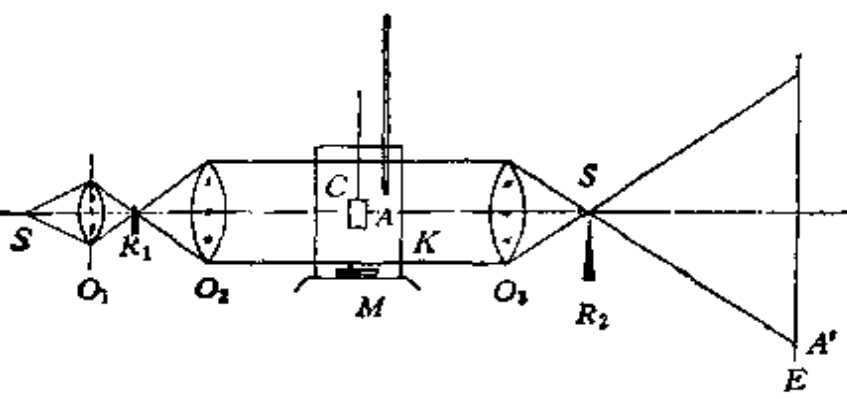
\includegraphics[width=0.8\textwidth]{fig/cp03/img3.9.jpg}
 \caption{测量溶液中不均匀区域的装置。}图中:$S$为光源;$O_1,O_2,O_3$为长焦距消色差透镜;$R$为可调的孔径光阑;$K$为透光面平行的测量槽;$C$为晶体;
 
 $M$为电磁搅拌器;$E$为屏幕。
\end{figure}
%Fig.3.9
其装置如图3.9所示。这种装置适用于观察透明介质中的局部光学不均匀性。光源$S$通过$O_1$,聚焦至可调孔径光栏$R_1$即$O_2$的焦点上,光线透过$O_2$即变成平行光照射到待测的不均匀透明介质上,经$O_3$成像于焦点$S'$,在该处放置一锐边遮光板或狭缝$R_2$,挡住了光源的像$S'$,因此在白色的屏幕上出现黑色的背景,但在$SS'$之间存在光学不均匀区域$A$,则光线发生偏折,从$R_2$的锐边旁通过在屏幕上给出其像$A'$。偏折方向与不均匀区域的折射率梯度方向有关。这种方法能发现折射率差别很小的不均匀区域。在光路中的待测生长池$K$中,晶体附近的不均匀扩散层可以在屏幕上清楚地显示出来。在不饱和的溶液中,扩散层的像出现在无遮光板一侧的晶体附近,在过饱和溶液中则恰好相反,如图3.9所示。当溶液到达饱和状态时,扩散层消失。在测定时,溶液可以不停地搅拌,生长池的温度可用电热吹风机调整。这种方法的精确度可达0.05℃,甚至更高。值得注意的是,光源应用单色光,用He-Ne激光更好,否则,$O_2,O_3$应用消色差透镜。

\subparagraph{(ii) 狭缝光源法}
该法是使一狭缝光源和置于待测溶液中晶体的一个晶面斜交,随着溶液状态的变化,在狭缝和晶面的交界处会出现不同的偏折现象,这也是由于存在扩散层这一光学上不均匀的区域所引起的。

\begin{figure}[htb]
 \centering
 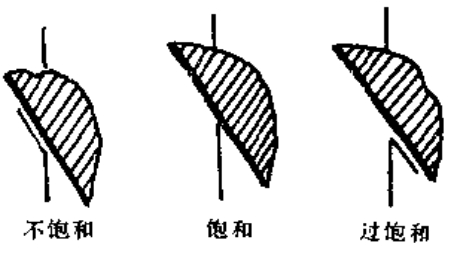
\includegraphics[width=0.6\textwidth]{fig/cp03/img3.10.jpg}
 \caption{狭缝光源在晶面交界处的光学效应。} 
\end{figure}
%Fig.3.10

当溶液不饱和时,明亮的狭缝在晶面交界处弯曲成钝角,当溶液为过饱和时,则向相反方弯曲成锐角。溶液愈偏离饱和状态,弯曲现象就越明显。随着溶液逐淅接近饱和,弯曲部分逐渐缩短,当溶液达到饱和时,狭缝光在晶面交界处不发生弯曲(图3.10)。根据这种现象所测定的饱和温度的精确度也可达到0.05℃。 使用这一方法时,可将盛有待测溶液的容器放在恒温槽中进行测量,也可通过特定装置将溶液从大育器中抽出,流过调温装置和测量装置,再泵浦回育晶器,这样可以迅速而准确地测定育晶器中溶液的饱和温度,在生产和实验室中使用这种方法是很方便的。

利用上述测定饱和温度的方法,特别是光学效应法,也可以进行溶解度的测定,并绘制出溶解度曲线。溶解度测定虽较简单,但需要有高度的实验技巧和精确度。

用平衡法测溶解度时,在到达平衡后应恒温静置使细小分散的固体颗粒沉降,仔细抽取一定量(不是一定体积)的溶液样品进行分析,确定溶液成分。溶液分析通常用重量法和容量法,有时也使用其他方法(如比色法以及密度、折射率、电导等方法)。溶液成分也可以预先准确配制(即称取一定量的溶剂和溶质),然后再测出溶液的饱和温度,确定其溶解度。

在确定溶液成分的同时,也有必要对与之相平衡的固相进行分析鉴定。有时在很小的温度区间内与饱和溶液相平衡的稳定相是可以改变的,转别是水合物体系。例如在0-100 ℃区间内测定$\rm Na_2CO_3$在水中的溶解度时发现,在32℃以下,其稳定相是$\rm Na_2CO_3\cdot 10H_2O$,而$\rm Na_2CO_3\cdot 7H_2O$在32.0℃到35.4℃之间稳定,$\rm Na_2CO_3\cdot H_2O$在35.4℃以上稳定。因此,必须将不同温度下的平衡固相晶体取出,在该温度下仔细于燥,并确定其成分。对于成分相同但结构不一样的不同晶相(多形体),还必须利用物理鉴定的方法来确定与溶液相平衡的物相。例如从高浓度重水($\rm D/(D+H)=99.8\%$)溶液中,生长磷酸二氘钾(DKDP)晶体时,DKDP会出现四方和单斜两种晶相。在21℃以下时,四方相是与溶液平衡的稳定相,在21℃以上时,单斜相是稳定相。这两相的溶解度十分接近(特别是在转变点附近),因此用通常测定溶解度的方法很难将它们区分开来。在这种情况下,光学效应法就显示出其优越性。图3.11示出的四方和单斜两相溶解度曲线就是用图3.9的装置测定出来的。对每一相不仅测定了在其相稳定区内(即稳定相)的溶解度曲线,还成功地测出了在另一相稳定区内(即亚稳相,参阅3.2.3节)的溶解度曲线,这样对四方相和单斜相都测出了一条完整的溶解度曲线。这两条曲线的交点即为DKDP溶解度曲线上的拐点,即四方相和单斜相的相平衡转变点(在图3.11中转变点为21 ℃)。
\begin{figure}[htb]
 \centering
 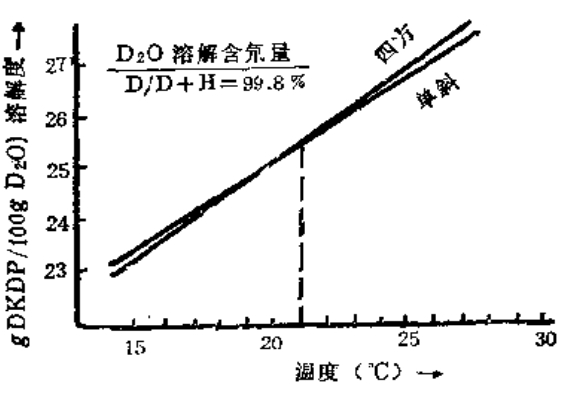
\includegraphics[width=0.6\textwidth]{fig/cp03/img3.11.jpg}
 \caption{DKDP的两相溶解度曲线。}
\end{figure}
%Fig.3.11
必须指出的是,在测定溶解度曲线的工作中,提高控温和测温的精度是十分重要的。例如在测定氯化钠在30℃水中的溶解度时,实验温度波动±0.5℃,引起溶解度测量误差约0.1\%,但在测定硫酸钠在30℃水中的溶解度时,同样的温度波动则能造成5\%的误差。所以在测定工作中,恒温器所用的温度计必须用标准温度计进行校正。

过饱和度是影响晶体生长速度和质量的重要因素,过饱和度的确定对晶体生长研究工作和培养单晶的实践都有重要意义。如果在给定温度下,溶液的浓度可以测量出来,而且相应的平衡饱和浓度是已知的,那么就不难根据式(3.7)---(3.9)来计算溶液的过饱和度。上述已提到,溶液浓度可以进行直接的分析,也可通过测量体系中某些对浓度变化敏感的性质(如密度、粘度、折射率和电导率等)来间接确定。在实验室的条件下,这些性质都可以测量得很精确。但在晶体培养过程中,要求在不破坏液体稳定性的条件下,能在育晶器中进行连续的测量。如果在生长过程中温度是变化的,还需知道被测量性质对温度的依赖关系,这样,问题就变得复杂了,因此直接应用还是较少。在上述对浓度敏感的性质中,密度和折射率对温度较不敏感。

溶液的过饱和度也可以用光学效应法在生长过程中直接测定,所得的过饱和度是以过冷度$\Delta t$表示的。这种方法的优点就是不需要知道溶液的准确成分和溶解度曲线,也不需改变育晶器的温度,在晶体生长过程中,任何时候都可测得溶液的真实过饱和度。遗憾的是,在晶体的生长过程中,抽取溶液进行循环流动,有破坏溶液稳定性,影响晶体生长的危险。但在三槽流动法中,对过热槽中的饱和度用上述方法进行测量则是十分安全和方便的。

各种过饱和度的测量方法,虽取得了一定的效果,但都存在着不少问题,有待于进一步研究解决,并希望能创造更简便、灵敏、可靠的能连续进行测量的新方法。